\documentclass[12pt, oneside]{book}
\usepackage[utf8]{inputenc}
\usepackage{graphicx}
\usepackage[slovak]{babel}
\usepackage{todonotes}
\usepackage{url}
\usepackage{listings}
\usepackage{amsfonts}
\usepackage{hyperref}
\usepackage[toc,page]{appendix}
\linespread{1.3}

\renewcommand{\lstlistingname}{Príkaz}
\renewcommand{\lstlistlistingname}{Zoznam príkazov}

\lstdefinestyle{karel}{
  belowcaptionskip=1\baselineskip,
  breaklines=true,
  frame=L,
  xleftmargin=\parindent,
  language=c,
  showstringspaces=false,
  basicstyle=\footnotesize\ttfamily,
  keywordstyle=\bfseries\color{green!40!black},
  commentstyle=\itshape\color{purple!40!black},
  identifierstyle=\color{blue},
  stringstyle=\color{red},
}

\lstset{escapechar=@,style=karel}

\colorlet{punct}{red!60!black}
\definecolor{background}{HTML}{EEEEEE}
\definecolor{delim}{RGB}{20,105,176}
\colorlet{numb}{magenta!60!black}

\setcounter{secnumdepth}{3}
\setcounter{tocdepth}{3}

% -------------------
% --- Definicia zakladnych pommov
% -------------------
\def\*{{\bf FIXME: }}
\def\mfyear{2016}
\def\mftitle{Inovácia prostredia Karel 3D a jeho využitie vo vyučovaní}
\def\mfthesistype{záverečná práca}
\def\mfauthor{Bc. Tomáš Kubla}
\def\mfadvisor{doc. PaedDr. Monika Tomcsányiová, PhD.}
\def\mfplacedate{Bratislava, \mfyear}
\def\odbor{2508 Informatika} %aj cislo odboru je povinne a je to podla katedry/odboru, na ktorom je autor
\def\program{ Informatika }
\def\stredisko{ Katedra informatiky }

\begin{document}     

% -------------------
% --- Obalka ------
% -------------------
\thispagestyle{empty}
\noindent

\begin{minipage}{0.95\textwidth}
\begin{center}
\sc  
\large
\vspace*{0.3cm} Univerzita Komenského v Bratislave\\
\vspace*{0.3cm} Fakulta matematiky, fyziky a informatiky\\
\end{center}
\end{minipage}

\vfill

\begin{minipage}{1.1\textwidth}
\begin{flushright}
\bigskip\bigskip
% tusim mam nadstandardne dlhy nazov :)
%\centerline{\sc\LARGE\mftitle}
\begin{center}
\sc\LARGE\mftitle
\end{center}
\centerline{\sc\mfthesistype}

\bigskip\bigskip\bigskip\bigskip
\end{flushright}
\end{minipage}
\vfill

\noindent \mfyear\\
\indent\mfauthor

\eject % EOP i
% --- koniec obalky ----

% -------------------
% --- Titulný list
% -------------------

\thispagestyle{empty}
\noindent

\begin{minipage}{0.95\textwidth}
\begin{center}
\sc  
\large
\vspace*{0.3cm} Univerzita Komenského v Bratislave\\
\vspace*{0.3cm} Fakulta matematiky, fyziky a informatiky\\
\end{center}
\end{minipage}

\vfill

\begin{minipage}{1.1\textwidth}
\begin{flushright}
\bigskip\bigskip
% tusim mam nadstandardne dlhy nazov :)
%\centerline{\sc\LARGE\mftitle}
\begin{center}
\sc\LARGE\mftitle
\end{center}
\centerline{\sc\mfthesistype}
\end{flushright}

\bigskip
\vspace{3cm}
\bigskip
\begin{tabular}{ll}  
Študijný program: & \program \\
Študijný odbor: & \odbor \\
Školiace pracovisko: & \stredisko \\
Školiteľ: & \mfadvisor \\
\end{tabular}
\todo[inline]{toto preverit, ci tam ma byt nieco ine, kedze sme dpsi}
\end{minipage}
\vfill

\noindent \mfplacedate\\
\indent\mfauthor

\eject % EOP i


% --- Koniec titulnej strany


% -------------------
% --- Naskenovane Zadanie
% -------------------
% v tlačenej verzii s podpismi zainteresovaných osôb.
% v elektronickej verzii sa zverejňuje zadanie bez podpisov zainteresovaných osôb.

\newpage 
\thispagestyle{empty}
%\hspace{-1cm}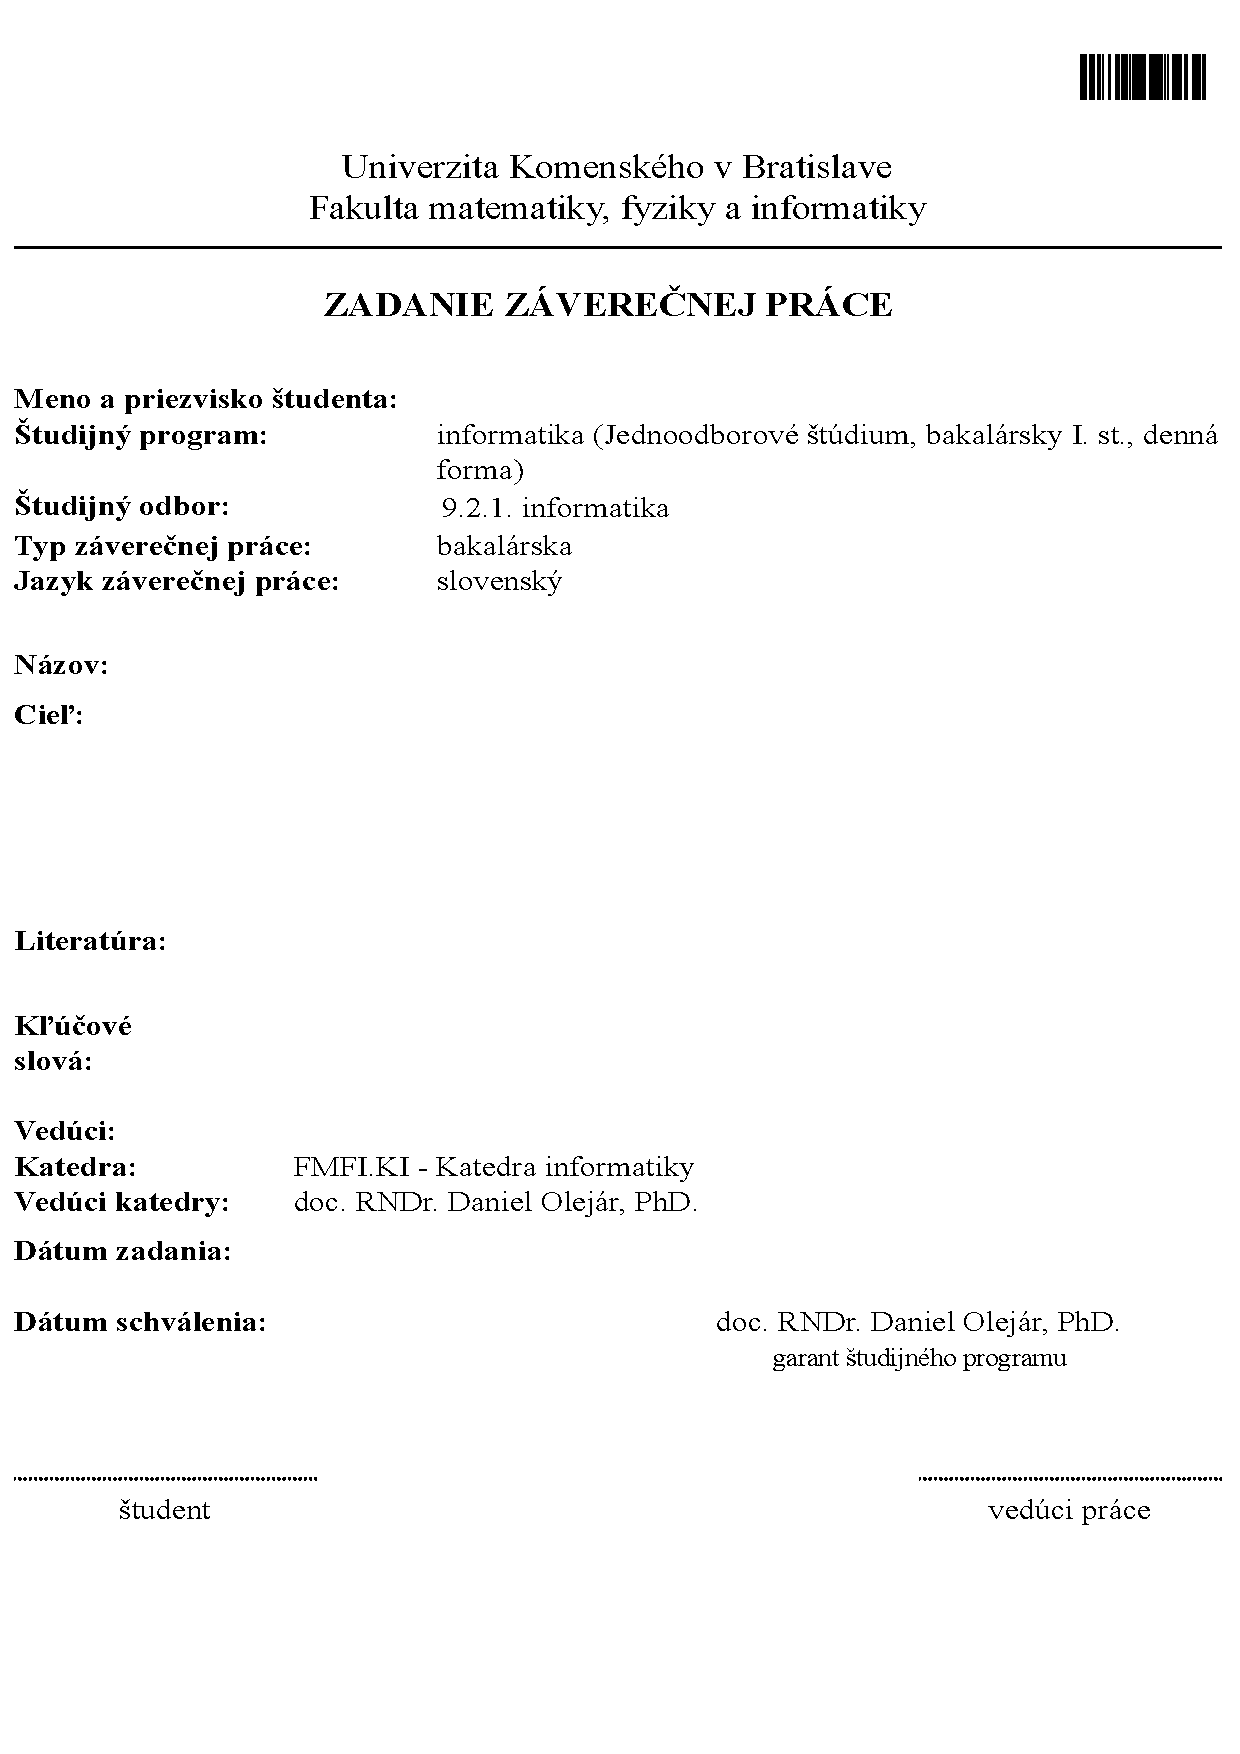
\includegraphics[width=1.2\textwidth]{images/zadanie}
\todo[inline]{dat sem zadanie}
% --- Koniec zadania

\frontmatter

% -------------------
%   Poďakovanie - nepovinné
% -------------------
\newpage 
\thispagestyle{empty}

\vfill
{\bf Poďakovanie:}

\input podakovanie.tex
% --- Koniec poďakovania

% -------------------
%   Abstrankt - Slovensky
% -------------------
\newpage 
\thispagestyle{empty}

\huge{Abstrakt}
\normalsize
\newline
Slovenský abstrakt 100-500 slov
\todo[inline]{spisat abstrakt}
{\bf Kľúčové slová:} jedno, druhé, tretie (prípadne štvrté, piate)
% --- Koniec Abstrakt - Slovensky


% -------------------
% --- Abstrakt - Anglicky 
% -------------------
\newpage 
\thispagestyle{empty}

\huge{Abstract}
\normalsize
\newline
English abstract
\todo[inline]{spisat abstrakt}

{\bf Keywords:} 

% --- Koniec Abstrakt - Anglicky

% -------------------
% --- Predhovor ?????
% -------------------
%\newpage 
%\thispagestyle{empty}
%
%\huge{Predhovor}
%\normalsize
%\newline
%Predhovor je všeobecná informácia o práci, obsahuje hlavnú charakteristiku práce 
%a okolnosti jej vzniku. Autor zdôvodní výber témy, stručne informuje o cieľoch 
%a význame práce, spomenie domáci a zahraničný kontext, komu je práca určená, 
%použité metódy, stav poznania; autor stručne charakterizuje svoj prístup a svoje 
%hľadisko. 
%
% --- Koniec Predhovor


% -------------------
% --- Obsah
% -------------------

\newpage 

\tableofcontents

% ---  Koniec Obsahu

% -------------------
% --- Zoznamy tabuliek, obrázkov
% -------------------

\newpage 

\listoffigures

\newpage

\lstlistoflistings

% ---  Koniec Zoznamov

\mainmatter


\input uvod.tex 

\input pedagogickezvasty.tex

\input prostredie.tex

\input metodika.tex

\input vyskum.tex

\input zaver.tex

% -------------------
% --- Bibliografia
% -------------------


\newpage	

\backmatter

\thispagestyle{empty}
\nocite{*}
\clearpage

\bibliographystyle{alpha}
\bibliography{literatura} 
%Prípadne môžete napísať literatúru priamo tu
%\begin{thebibliography}{5}
 
%\bibitem{br1} MOLINA H. G. - ULLMAN J. D. - WIDOM J., 2002, Database Systems, Upper Saddle River : Prentice-Hall, 2002, 1119 s., Pearson International edition, 0-13-098043-9

%\bibitem{br2} MOLINA H. G. - ULLMAN J. D. - WIDOM J., 2000 , Databasse System implementation, New Jersey : Prentice-Hall, 2000, 653s., ???

%\bibitem{br3} ULLMAN J. D. - WIDOM J., 1997, A First Course in Database Systems, New Jersey : Prentice-Hall, 1997, 470s., 

%\bibitem{br4} PREFUSE, 2007, The Prefuse visualization toolkit,  [online] Dostupné na internete: <http://prefuse.org/>

%\bibitem{br5} PREFUSE Forum, Sourceforge - Prefuse Forum,  [online] Dostupné na internete: <http://sourceforge.net/projects/prefuse/>

%\end{thebibliography}

%---koniec Referencii

% -------------------
%--- Prilohy---
% -------------------

\begin{appendices}
%Nepovinná časť prílohy obsahuje materiály, ktoré neboli zaradené priamo  do textu. Každá príloha sa začína na novej strane.
%Zoznam príloh je súčasťou obsahu.
%
%\addcontentsline{toc}{chapter}{Appendix A}
%\input AppendixA.tex
%
%\addcontentsline{toc}{chapter}{Appendix B}
%\input AppendixB.tex

\input priloha_cinanek.tex
\end{appendices}
\end{document}
